% =====================================================================
% EXPERIMENTACIÓN PROPIA.
%  1. Justifica: Netflix no se puede ejecutar localmente; usaste Eureka, que es de Netflix OSS.
%  2. Describe el montaje (Docker Compose, 1 Eureka + 3 copias de servicio-catalogo, puertos).
%  3. Describe el procedimiento (docker kill, sondeo cada 2 s, docker start). Los comandos están en el repositorio.
%  4. Presenta los resultados (tabla) y las capturas.
%  5. INTERPRETA con los conceptos de la sección anterior: ¿por qué tardó ~30 s y no 15?
%     ¿qué pasaba con un cliente durante esos 30 s? ¿qué dice esto de CAP? ¿por qué la
%     recuperación fue más rápida que la detección?
% =====================================================================
\section{Experimentación propia}

\textit{[Escribe aquí la justificación y el montaje del experimento.]}

\begin{figure}[H]
  \centering
  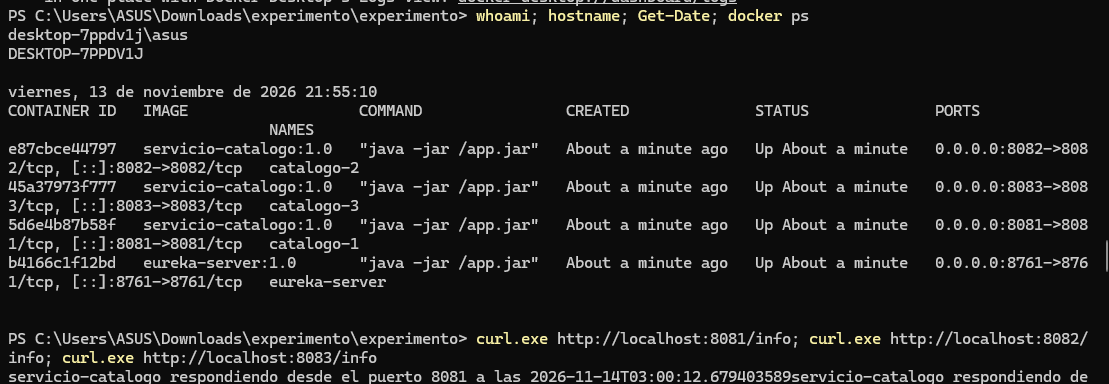
\includegraphics[width=0.85\textwidth]{01-docker-ps.png}
  \caption{Contenedores de Eureka y de las tres copias de \texttt{servicio-catalogo} en ejecución.}
  \label{fig:dockerps}
\end{figure}

\begin{figure}[H]
  \centering
  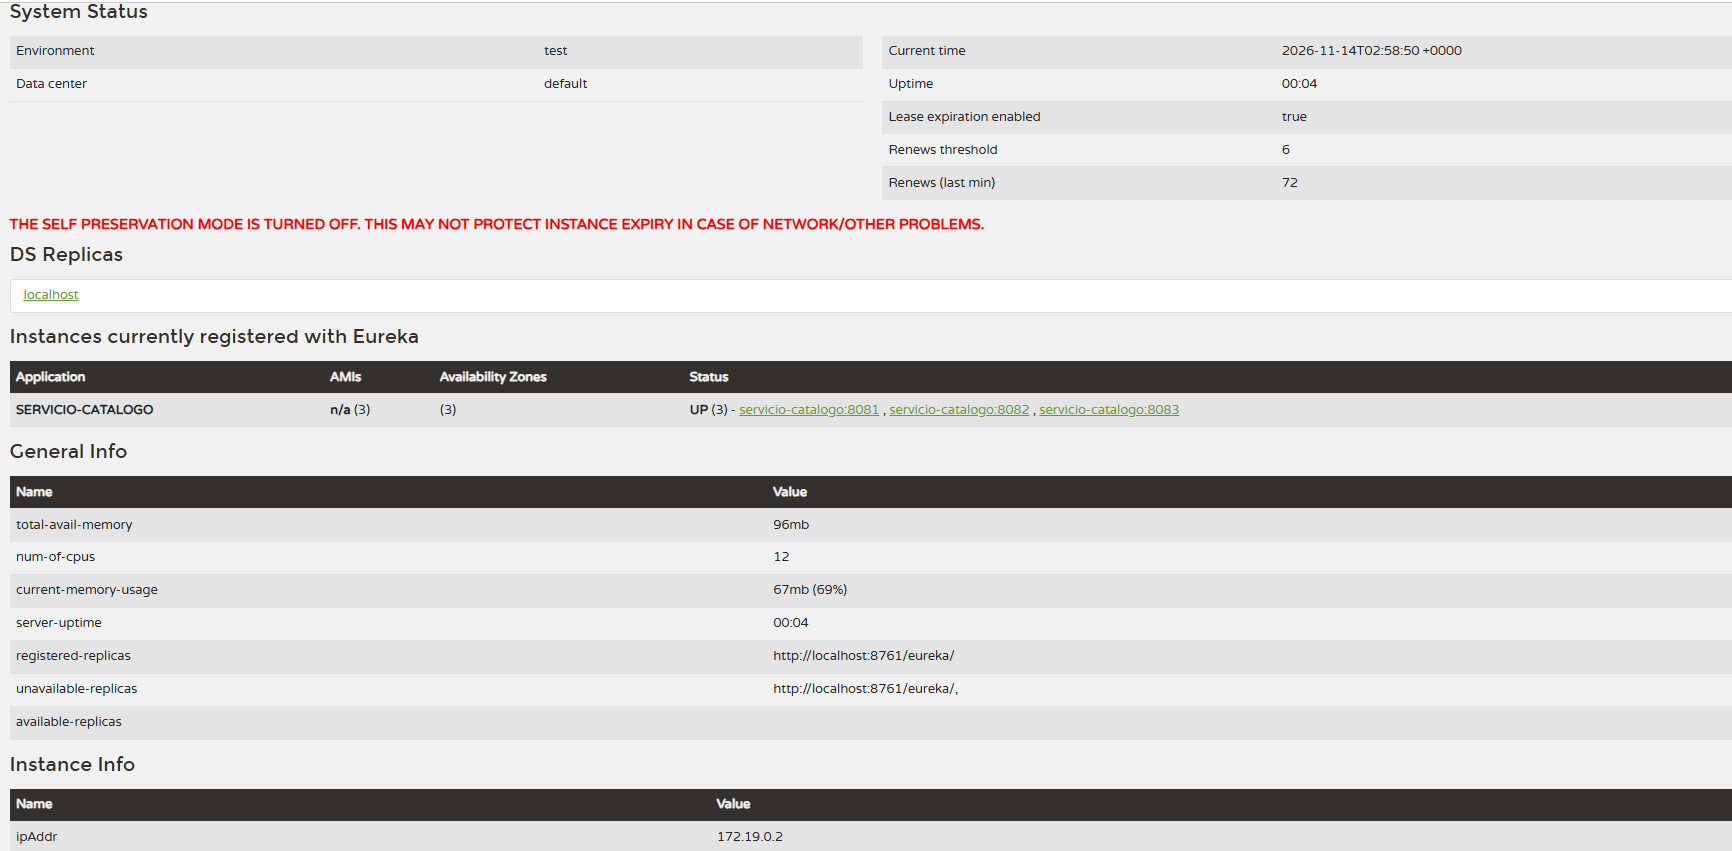
\includegraphics[width=0.95\textwidth]{02-eureka-panel.png}
  \caption{Panel de Eureka con las tres instancias de \texttt{SERVICIO-CATALOGO} en estado UP.}
  \label{fig:eureka}
\end{figure}

\begin{figure}[H]
  \centering
  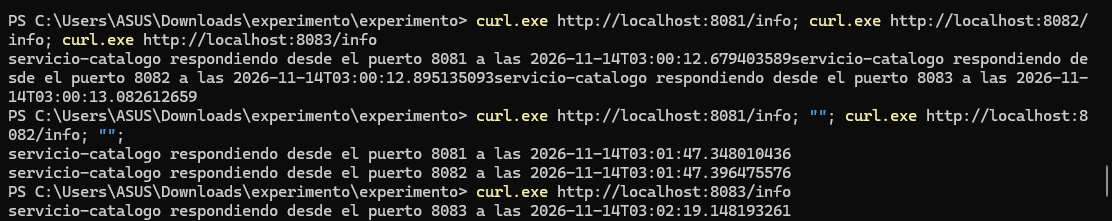
\includegraphics[width=0.85\textwidth]{03-curl-3-copias.png}
  \caption{Respuesta de las tres copias del servicio.}
  \label{fig:curl3}
\end{figure}

\textit{[Escribe aquí el procedimiento de la caída y la recuperación.]}

\begin{figure}[H]
  \centering
  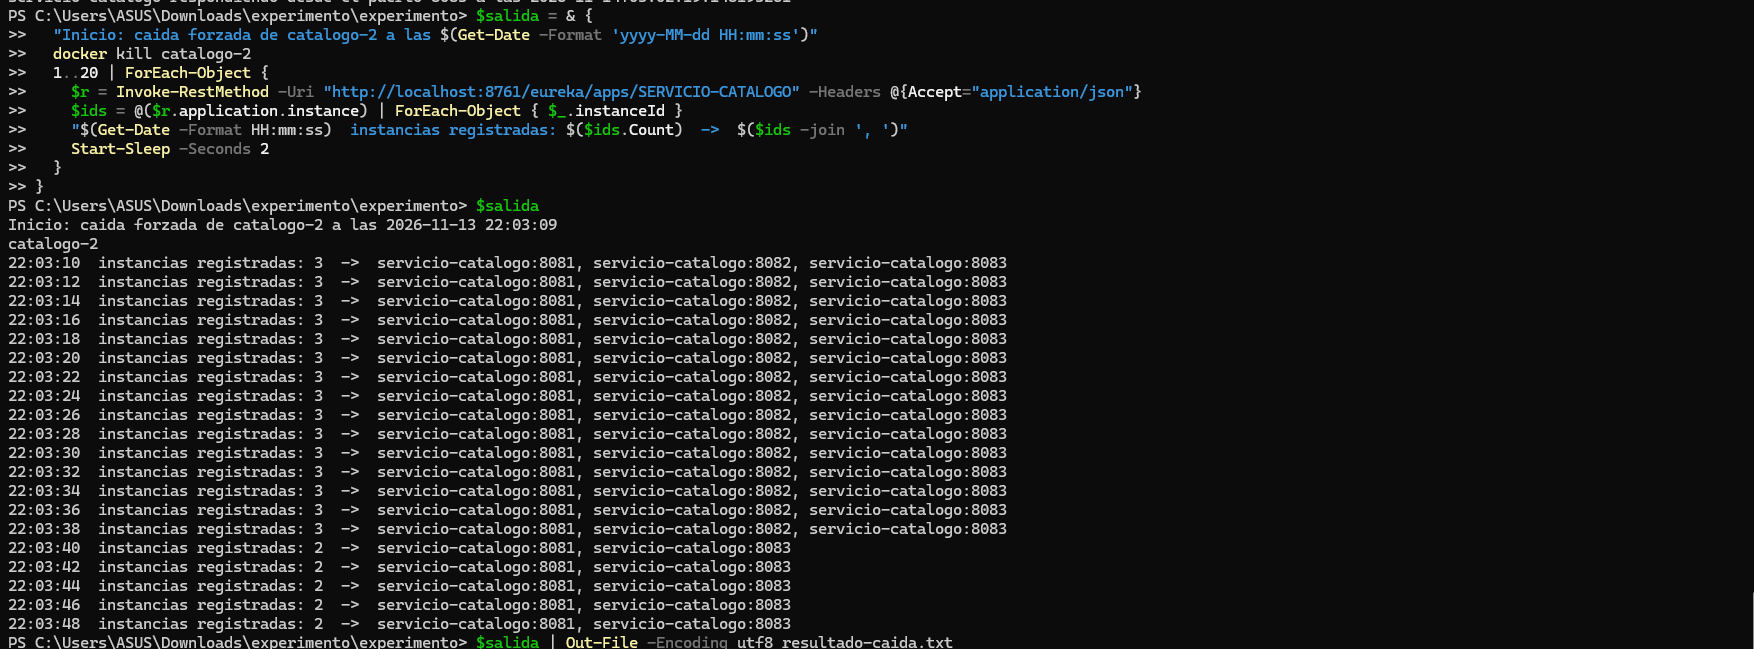
\includegraphics[width=0.95\textwidth]{04-caida.png}
  \caption{Caída forzada de \texttt{catalogo-2} y sondeo del registro de Eureka cada 2 s.}
  \label{fig:caida}
\end{figure}

\begin{figure}[H]
  \centering
  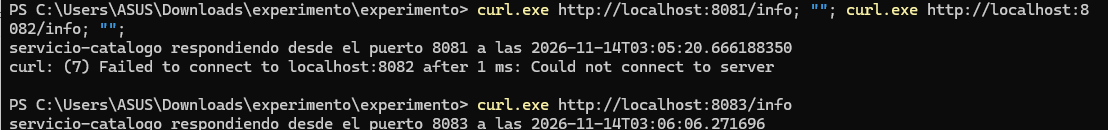
\includegraphics[width=0.85\textwidth]{05-curl-falla-8082.png}
  \caption{El puerto 8082 deja de responder mientras 8081 y 8083 siguen atendiendo.}
  \label{fig:falla8082}
\end{figure}

\begin{figure}[H]
  \centering
  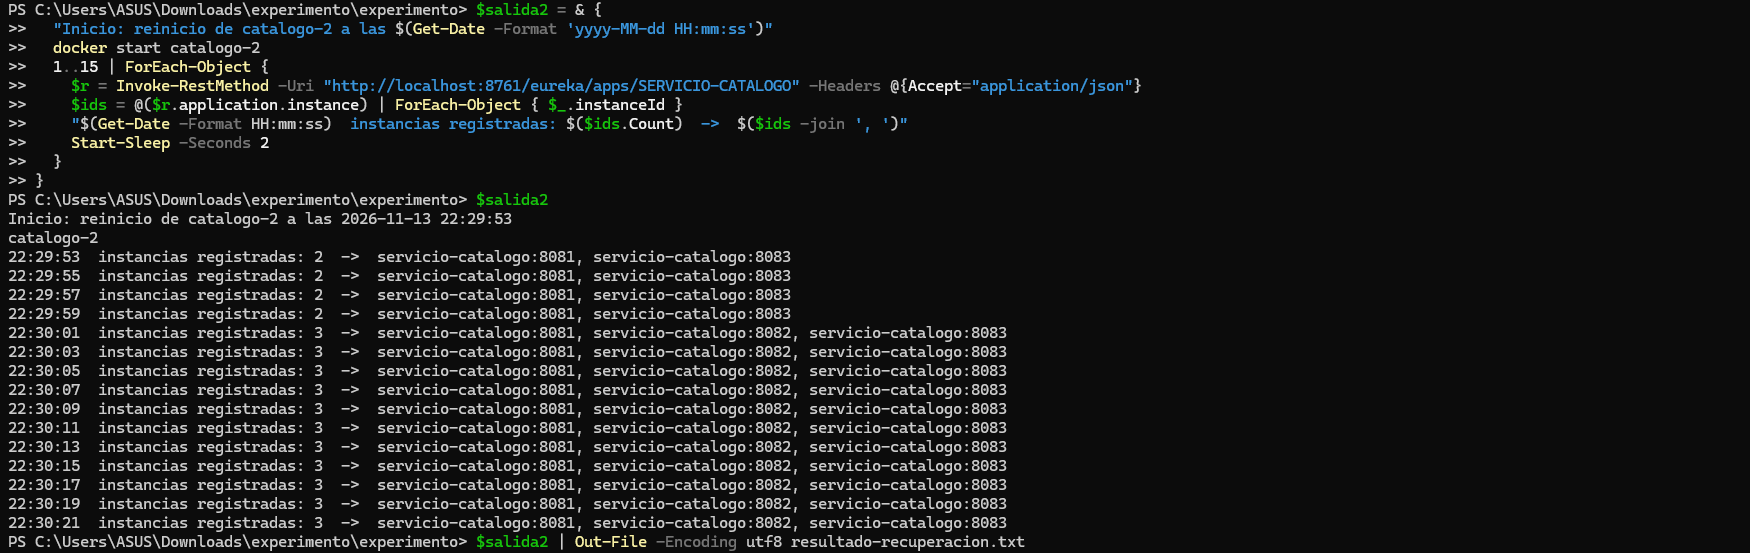
\includegraphics[width=0.95\textwidth]{06-recuperacion.png}
  \caption{Reinicio de \texttt{catalogo-2} y su vuelta al registro de Eureka.}
  \label{fig:recuperacion}
\end{figure}

\begin{table}[H]
  \centering
  \caption{Resultados del experimento (13 de noviembre de 2026).}
  \label{tab:resultados}
  \begin{tabular}{lccc}
    \toprule
    Evento & Inicio & Cambio en Eureka & Tiempo aprox. \\
    \midrule
    Caída de \texttt{catalogo-2} (\texttt{docker kill}) & 22:03:09 & 3 $\rightarrow$ 2 a las 22:03:40 & 30 s \\
    Reinicio de \texttt{catalogo-2} (\texttt{docker start}) & 22:29:53 & 2 $\rightarrow$ 3 a las 22:30:01 & 8 s \\
    \bottomrule
  \end{tabular}
\end{table}

\textit{[Escribe aquí la interpretación de los resultados.]}
